%\documentclass[preprint,tightenlines,showpacs,showkeys,floatfix,
%nofootinbib,superscriptaddress,fleqn]{revtex4} 
\documentclass[floatfix,nofootinbib,superscriptaddress,fleqn]{revtex4-2} 
%\documentclass[aps,epsfig,tightlines,fleqn]{revtex4}
\usepackage{kotex}
\usepackage[HWP]{dhucs-interword}
\usepackage[dvips]{color}
\usepackage{graphicx}
\usepackage{bm}
%\usepackage{fancyhdr}
%\usepackage{dcolumn}
\usepackage{defcolor}
\usepackage{amsmath}
\usepackage{amsfonts}
\usepackage{amssymb}
\usepackage{amscd}
\usepackage{amsthm}
\usepackage[utf8]{inputenc}
%\pagestyle{fancy}

\begin{document}

\title{\Large Quantum Mechanics}
\author{김현철}
\email{hchkim@inha.ac.kr}
\affiliation{Hadron Theory Group, Department of Physics, Inha University,
Incheon 22212, Republic of Korea }
\date{2021}

\maketitle

\noindent {\bf Due date:} \textbf{\color{red} March 2. 2022} \\ 
\vspace{2cm}

\section*{\large Problem Set 1}
\noindent \textbf{Problem 1.}
The wave function for a free particle is given by
\begin{align*}
\psi(x,\,0) = N \exp\left( i\frac{p_0 x}{\hbar}  
-\frac{(x-x_0)^2}{4\sigma^2} \right),   
\end{align*}
where $\sigma \in \mathbb{R}$ is a contant and $N$ is a normalization
constant. 
\begin{itemize}
\item[(1)] Derive the normalization constant $N$.  
\item[(2)] Derive the wave function $\phi(0,\,0)$ in momentum space. 
\item[(3)] Find $\phi(p,\,t)$.
\item[(4)] Find $\psi(x\,t)$.
\item[(5)] Show that the the spread in the spatial probability
  distribution increases with time $t$. Note that the spread is
  defined as 
  \begin{align*}
\mathcal{S}(t) = \frac{|\psi(x,\,t)|^2}{|\psi(0,t)|^2}.    
  \end{align*}
\end{itemize}
\noindent \textbf{Solution : }
\begin{itemize}
  \item[(1)] From the normalization of the wave function,
  \begin{align*}
    \int_{-\infty}^{\infty} |\psi(x,0)|^2\,dx=N^2\int_{-\infty}^{\infty}
    \exp\left(-2{\left(\frac{x-x_0}{2\sigma}\right)}^2\right) \,dx =1.
  \end{align*}
Since a range of integration is all space, the translation 
about $x$ can be ignored.
To make a compact form, it needs to change an integral variable.
  \begin{align*}
    t \equiv \left(\frac{x-x_0}{\sqrt{2}\sigma}\right),\;\;\; dt 
    = \frac{1}{\sqrt{2}\sigma} dx 
  \end{align*}
Then the wave function changes into more comfort form to integrate.
  \begin{align}\label{eq:gt}
    \int_{-\infty}^{\infty}\exp\left(-2{\left(
      \frac{x-x_0}{2\sigma}\right)}^2\right) \,dx
    =\sqrt{2}\sigma \int_{-\infty}^{\infty} e^{-t^2} \,dt
  \end{align}
To calcualte this integration, we use a idea of double integration,
  \begin{align*}
    \begin{split} 
      \int_{-\infty}^{\infty} e^{-(x^2+y^2)}\,dx\,dy 
      &= \int_{0}^{2\pi}\int_{0}^{\infty} e^{-r^2}r\,dr\,d\theta
      \\   &= \int_{0}^{2\pi}\frac{1}{2}\,d\theta = \pi.
    \end{split}
  \end{align*}
First double integration about coordinate space can be decomposed.
  \begin{align*}
    \int_{-\infty}^{\infty} e^{-(x^2+y^2)}\,dx\,dy 
    = \int_{-\infty}^{\infty} e^{-x^2}\,dx\int_{-\infty}^{\infty}e^{-y^2}\,dy
    = \left(\int_{-\infty}^{\infty} e^{-x^2}\,dx\right)^2
  \end{align*}
From this result,
  \begin{align*}
    \int_{-\infty}^{\infty} e^{-x^2} \,dx 
    = \sqrt{\pi},\quad \sqrt{2\pi}\sigma N^2 =1.
  \end{align*}
Finally we obtain the normalization constant,
  \begin{align}
    \,N = {\left(\frac{1}{2\pi\sigma^2}\right)}^{\frac{1}{4}}.
  \end{align}
  \item[(2)]  We will find $\phi(p,0)$ first. 
  $\phi(p,0)$ is the Fourier transform of $\psi(x,0)$.
  \begin{align*}
    \begin{split} 
      \phi(p,0)=\frac{1}{\sqrt{2\pi\hbar}}
      \int\psi(x,0) e^{-\frac{i}{\hbar}px}\,dx
      =\frac{N}{\sqrt{2\pi\hbar}}
      \int\exp\left(i\frac{p_0 x}{\hbar}-{\left(
        \frac{x-x_0}{2\sigma}\right)}^2\right) 
        e^{-\frac{i}{\hbar}px}\,dx  \\
        =\frac{N}{\sqrt{2\pi\hbar}}
        \int\exp\left(-{\left(\frac{x-x_0}{2\sigma}\right)}^2
        -\frac{i}{\hbar}(p-p_0)x\right)\,dx
      \end{split}
  \end{align*}
  To make it compact form, let us erase the translation term 
  and change the variable.
  \begin{align*}
    u \equiv \frac{x-x_0}{2\sigma},\;\;\; du = \frac{1}{2\sigma} dx 
  \end{align*}
  Then, a $\phi(p,0)$ is,
  \begin{align*}
    \begin{split}
      \phi(p,0)&=\frac{2\sigma N}{\sqrt{2\pi\hbar}}
      \int\exp\left(-{u}^2-\frac{i}{\hbar}(p-p_0)(2\sigma u+x_0)\right)\,du \\
      &={\left(\frac{2\sigma^2}{\pi^3\hbar^2}\right)}^{\frac{1}{4}}
      e^{-\frac{i}{\hbar}(p-p_0)x_0}
      \int\exp\left(-u^2-2\frac{i}{\hbar}\sigma (p-p_0)u\right)\,du.
    \end{split}
  \end{align*}
  And, a exponential of integrated function can be expressed 
  in terms of complete square form about u.
  \begin{align}
    -u^2-2\frac{i}{\hbar}\sigma (p-p_0)u 
    = -{\left( u+\frac{i}{\hbar}\sigma (p-p_0)\right)}^2
    -\frac{\sigma^2}{\hbar^2}{(p-p_0)}^2
  \end{align}
  $\frac{i}{\hbar}\sigma p$ is the translation term that can be ignored 
  since the integration range is from $-\infty$ to $\infty$,
  \begin{align*}
    \begin{split}  
      \phi(p,0) &= {\left(\frac{2\sigma^2}{\pi^3\hbar^2}\right)}^{\frac{1}{4}}
      e^{-\frac{i}{\hbar}(p-p_0)x_0}
      \int\exp\left(-u^2-2\frac{i}{\hbar}\sigma (p-p_0)u\right)\,du \\
      &={\left(\frac{2\sigma^2}{\pi^3\hbar^2}\right)}^{\frac{1}{4}}
      e^{-\frac{i}{\hbar}(p-p_0)x_0}  
      \int\exp\left(-{\left( u+\frac{i}{\hbar}\sigma (p-p_0)\right)}^2
      -\frac{\sigma^2}{\hbar^2}(p-p_0)^2\right)\,du \\
      &= {\left(\frac{2\sigma^2}{\pi^3\hbar^2}\right)}^{\frac{1}{4}}
      \exp\left( -\frac{i}{\hbar}(p-p_0)x_0
      -\frac{\sigma^2}{\hbar^2}(p-p_0)^2 \right)
      \int e^{-u^2}\,du
    \end{split}
  \end{align*}
  So, we obtain a $\phi(p.0)$.
  \begin{align*}
    \begin{split}
      \phi(p,0) &= {\left(\frac{2\sigma^2}{\pi^3\hbar^2}\right)}
      ^{\frac{1}{4}}
      \exp\left( -\frac{i}{\hbar}(p-p_0)x_0
      -\frac{\sigma^2}{\hbar^2}(p-p_0)^2 \right)
      \int e^{-u^2}\,du \\
      &= {\left(\frac{2\sigma^2}{\pi\hbar^2}\right)}^{\frac{1}{4}}
      \exp\left( -\frac{i}{\hbar}(p-p_0)x_0
      -\frac{\sigma^2}{\hbar^2}(p-p_0)^2 \right)
    \end{split}
  \end{align*}
  Finally, $\phi(0,0)$ is,
  \begin{align}
    \phi(0,0) = {\left(\frac{2\sigma^2}{\pi\hbar^2}\right)}^{\frac{1}{4}}
    \exp\left(-\frac{\sigma^2}{\hbar^2}{p_0}^2+\frac{i}{\hbar}p_0x_0\right).
  \end{align}
  \item[(3)]Because it is a free particle, the time evolution of 
  $\phi(p,0)$ is $\phi(p,t)=e^{-i\omega t}\phi(p,0)$ 
  and $\omega = \frac{p^2}{2m\hbar}$.
  \begin{align*}
      \phi(p,t) &={\left(\frac{2\sigma^2}{\pi\hbar^2}\right)}^{\frac{1}{4}}
      \exp\left(-\frac{\sigma^2}{\hbar^2}(p-p_0)^2-i\frac{p^2}{2m\hbar}t
      -\frac{i}{\hbar}(p-p_0)x_0 \right) \\
      &={\left(\frac{2\sigma^2}{\pi\hbar^2}\right)}^{\frac{1}{4}}
      \exp\left(-\left(\frac{\sigma^2}{\hbar^2} 
      +\frac{it}{2m\hbar}\right)p^2 
      +\left(\frac{2\sigma^2}{\hbar^2}p_0-\frac{i}{\hbar}x_0\right)p 
      -\frac{\sigma^2}{\hbar^2}p_0^2+\frac{i}{\hbar}p_0x_0 \right) \\ 
      &={\left(\frac{2\sigma^2}{\pi\hbar^2}\right)}^{\frac{1}{4}}
      \exp\left(-\frac{2m\sigma^2+i\hbar t}{2m\hbar^2}p^2 
      +\frac{2\sigma^2p_0-i\hbar x_0}{\hbar^2}p
      -\frac{\left(\sigma^2p_0-i\hbar x_0\right)p_0}{\hbar^2} \right)
  \end{align*}
  \item[(4)] $\psi(x,t)$ is the Fourier transform of $\phi(p,t)$.
  \begin{align}
    \begin{split}
      \psi(x,t) &= \frac{1}{\sqrt{2\pi\hbar}}
      \int\phi(p,t)e^{\frac{i}{\hbar}px}\,dp  \\
      &={\left(\frac{\sigma^2}{2\pi^3\hbar^4}\right)}^{\frac{1}{4}}
      \int\exp\left(-\frac{2m\sigma^2+i\hbar t}{2m\hbar^2} p^2 
      +\frac{2\sigma^2p_0+i\hbar (x-x_0)}{\hbar^2}p
      -\frac{\left(\sigma^2p_0-i\hbar x_0\right)p_0}{\hbar^2}\right)\,dp  \\
      &={\left(\frac{\sigma^2}{2\pi^3\hbar^4}\right)}^{\frac{1}{4}}
      \int\exp{\left( -\alpha(t)p^2+\beta(x)p+\gamma\right)}\,dp
    \end{split}
  \end{align}
  $\alpha(t)$, $\beta(t)$ and $\gamma(x,t)$ are the replacement factors that,
  \begin{align}
    \begin{split}\label{eq:abg}
      &\alpha(t) =\frac{2m\sigma^2+i\hbar t}{2m\hbar^2},\,\,\,
    \beta(t) =\frac{2\sigma^2p_0+i\hbar(x-x_0)}{\hbar^2},\,\,\,
    \gamma=\frac{\left(\sigma^2p_0-i\hbar x_0\right)p_0}{\hbar^2} \\
    \end{split}
  \end{align}
  This integration is a type of guassian integration.
  \begin{align}
    \begin{split}
      \int\exp{\left( -\alpha(t)p^2+\beta(x)p+\gamma\right)}\,dp
      =\sqrt{\frac{\pi}{\alpha(t)}}
      \exp\left(\frac{(\beta(x))^2}{4\alpha(t)}-\gamma\right)
    \end{split}
  \end{align}
  Finally, we obtain $\psi(x,t)$,
  \begin{align}
    \psi(x,t) &= {\left(\frac{\sigma^2}{2\pi\hbar^4}\right)}^{\frac{1}{4}}
    \sqrt{\frac{1}{\alpha(t)}}
    \exp\left(\frac{(\beta(x))^2}{4\alpha(t)}-\gamma\right) \\
    &={\left(\frac{\sigma^2}{2\pi}\right)}^{\frac{1}{4}}
    \sqrt{\frac{2m}{2m\sigma^2+i\hbar t}}
    \exp\left(\frac{m\left(2\sigma^2p_0
    +i\hbar(x-x_0)^2\right)\left(2m\sigma^2-i\hbar t\right)}
    {2\hbar^2\left(4m^2\sigma^4+\hbar^2 t^2\right)}
    -\frac{\left(\sigma^2p_0-i\hbar x\right)p_0}{\hbar^2}\right)
  \end{align}
  \item[(5)] Set $\hbar = 1$. Then the probability density is,
  \begin{align}
    \begin{split}
      |\psi(x,t)|^2 &= {\left(\frac{\sigma^2}{2\pi}\right)}^{\frac{1}{2}}
      \frac{2m}{\sqrt{4m^2\sigma^4+t^2}}
      \exp\left(
        \frac{2m^2\sigma^2\left(4\sigma^4p_0^2
        -\left(x-x_0\right)^2\right)
        +4m\sigma^2p_0(x-x_0)t}
        {4m^2\sigma^4+t^2}
        -2\sigma^2p_0^2\right)  \\
      &= {\left(\frac{\sigma^2}{2\pi}\right)}^{\frac{1}{2}}
      \frac{2m}{\sqrt{4m^2\sigma^4+t^2}}
      \exp\left(
        \frac{k(x)
        +4m\sigma^2p_0(x-x_0)t}
        {4m^2\sigma^4+t^2}
        -2\sigma^2p_0^2\right), 
      \end{split}
  \end{align}
  and $k(x)$ is the replacement factor,
  \begin{align}
    k(x) = 2m^2\sigma^2\left(4\sigma^4p_0^2
    -\left(x-x_0\right)^2\right).
  \end{align}
  The spread is,
  \begin{align}
    \mathcal{S}(t) = \frac{|\psi(x,\,t)|^2}{|\psi(x,0)|^2}
    = \sqrt{\frac{4m^2\sigma^4}{4m^2\sigma^4+t^2}}
    \exp\left(
      \frac{k(x)
    +4m\sigma^2p_0(x-x_0)t}
    {4m^2\sigma^4+t^2}
    -\frac{k(x)}
    {4m^2\sigma^4}
    \right)
  \end{align}
Suppose that $\sigma = 0.6$, $m=2$, $x_0=2$ and $p_0=2$. Through the 
FIG. \ref{pic:1-1} and FIG. \ref{pic:1-2}, we can confirm that 
$|\psi|^2$ is spread and the spread $\mathcal{S}(t)$ is 
increases with time t.
  \begin{figure}[htbp]
    \centering
    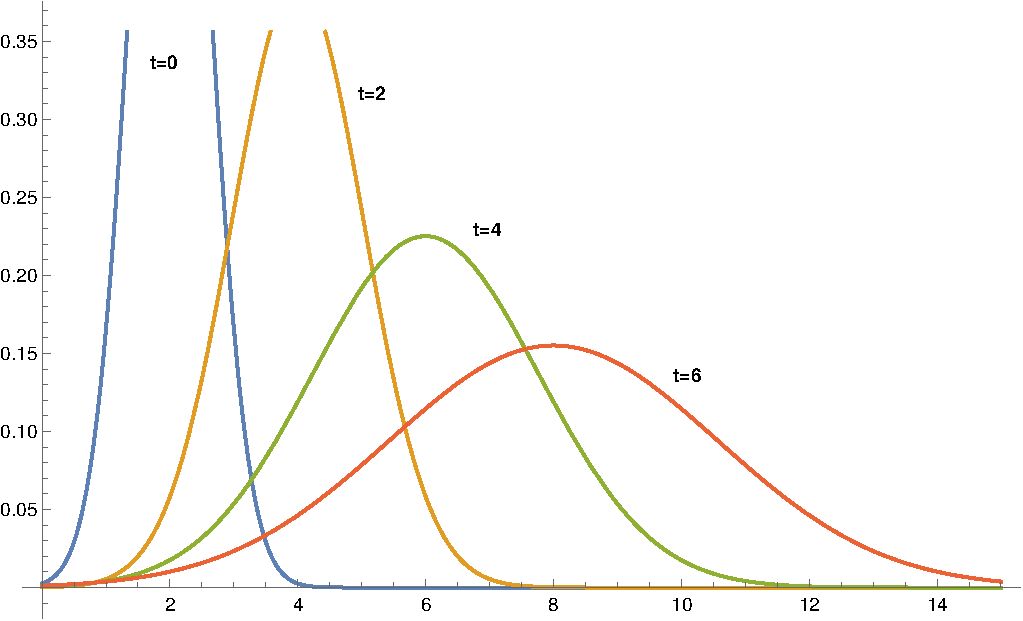
\includegraphics[scale=0.6]{1.pdf}  
    \caption{Normalized $|\psi|^2$ in different time}
    \label{pic:1-1}
    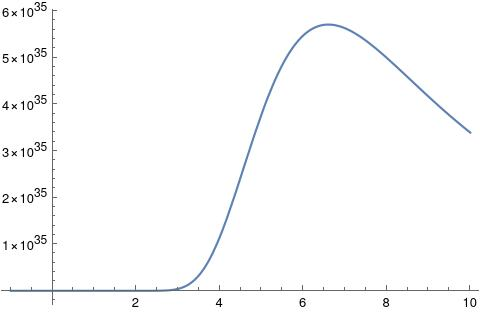
\includegraphics[scale=0.6]{2.jpg} 
    \caption{$\mathcal{S}(t)$ with $x=10$}
    \label{pic:1-2}
  \end{figure}
\end{itemize}
\vspace{0.5cm}

\noindent \textbf{Problem 2.} 
The Hamiltonian for a free particle is given by
\begin{align*}
H  = \frac{p^2}{2m}.
\end{align*}
\begin{itemize}
\item[(1)] Show 
  \begin{align*}
    \langle p_x \rangle = \langle p_x\rangle_{t=0}.
  \end{align*}
\item[(2)] Show 
  \begin{align*}
    \langle x \rangle = \frac{\langle p_x\rangle_{t=0}}{m} t + \langle
    x \rangle_{t=0}.
  \end{align*}
\item[(3)] Show 
  \begin{align*}
(\Delta p_x)^2 =  (\Delta p_x)_{t=0}^2  .
  \end{align*}
\item[(4)] Find $d(\Delta x)^2/dt$ as a function of time and initial 
  conditions. 
\end{itemize}

\noindent \textbf{Solution : }
\begin{itemize}
  \item[(1)]The expectation value of physical quantity can be 
  expressed in coordinate space and momentum space each other.
  For free particle, the $\phi(p,t)$ is,
  \begin{align}\label{phi:te}
    \phi(p,t)=e^{-i\frac{p^2}{2m\hbar}t}\phi(p,0)  .
  \end{align}
  And the expectation value of $p_x$ in the momentum space is,
  \begin{align*}
    \langle p_x \rangle &= \int \phi^*(p,t)\,p_x\,\phi(p,t)\,d^3p
    =\int e^{i\frac{p^2}{2m\hbar}t}\phi^*(p,0)\,p_x\,
    e^{-i\frac{p^2}{2m\hbar}t}\phi(p,0)\,d^3p
  \end{align*}
  The time evolutions are canceled out.
  \begin{align}\label{thm:px}
    \langle p_x \rangle=\int \phi^*(p,0)\,p_x\,\phi(p,0)\,d^3p 
    = \langle p_x \rangle_{t=0}.
  \end{align}
  \item[(2)] The expectation value of $x$ also can be described in 
  the momentum space regarding as the operator in the integration.
  \begin{align}
    \begin{split}
      \langle x\rangle &= i\hbar\int \phi^*(p,t)
      \frac{\partial\phi(p,t)}{\partial p_x}\,d^3p 
    =i\hbar\int e^{i\frac{p^2}{2m\hbar}t}\phi^*(p,0)
    \frac{\partial}{\partial p_x}\left(e^{-i
    \frac{p^2}{2m\hbar}t}\phi(p,0)\right)\,d^3p  \\
    &=i\hbar\int e^{i\frac{p^2}{2m\hbar}t}\phi^*(p,0)
    \left(-i\frac{p_x}{m\hbar}t\,e^{-i\frac{p^2}{2m\hbar}t}\phi(p,0)
    +e^{-i\frac{p^2}{2m\hbar}t}
    \frac{\partial \phi(p,0)}{\partial p_x}\right)\,d^3p \\
    &=i\hbar\int -i\frac{p_x}{m\hbar}t\,|\phi(p,0)|^2
    +\phi^*(p,0)\frac{\partial \phi(p,0)}{\partial p_x}\,d^3p \\
    &=\frac{\langle p_x\rangle_{t=0}}{m}t+\langle x\rangle_{t=0} 
    \end{split}
  \end{align}
  \item[(3)] The definition of the deviation is,
  \begin{align}\label{def:deviation}
    (\Delta p_x)^2 = \langle p_x^2 \rangle-\langle p_x \rangle^2. 
  \end{align}
  We calculate $\langle p_x^2 \rangle$ in the momentum space 
  and $\langle p_x \rangle^2=\langle p_x \rangle^2_{t=0}$ because 
  of (\ref{thm:px}).
  \begin{align*}
    \begin{split}
      \langle p_x^2 \rangle &= \int \phi^*(p,t)\,p^2_x\,\phi(p,t)\,d^3p
    \end{split}
  \end{align*}
  From (\ref{phi:te}),
  \begin{align*}
    \begin{split}
      \int \phi^*(p,t)\,p^2_x\,\phi(p,t)\,d^3p
      &=\int e^{i\frac{p^2}{2m\hbar}t}\phi^*(p,0)p^2_x 
      e^{-i\frac{p^2}{2m\hbar}t}\phi(p,0)\,d^3p  \\
      &=\int\phi^*(p,0)p^2_x\phi(p,0)\,d^3p =\langle p^2_x \rangle_{t=0}
    \end{split}      
  \end{align*}
  So, we obtain that,
  \begin{align}
    \langle p_x^2 \rangle=\langle p_x^2 \rangle_{t=0}.
  \end{align}
Finally, the result is,
\begin{align}
  (\Delta p_x)^2 = \langle p_x^2\rangle_{t=0}
  -\langle p_x \rangle^2_{t=0}
  =(\Delta p_x)^2_{t=0}, 
  \,\,\, (\Delta p_x)^2=(\Delta p_x)^2_{t=0}. 
\end{align}
  \item[(4)] From (\ref{def:deviation}), the derivative of the deviation is,
  \begin{align}
    \frac{d}{dt}(\Delta x)^2=\frac{d}{dt}\langle x^2\rangle
    -\frac{d}{dt}\left(\langle x \rangle^2\right). 
  \end{align}
  Before derivation, let us calculate the expectation value 
  $\langle x^2 \rangle$ first.
  \begin{align*}
    \begin{split}  
      \langle x^2 \rangle =& -\hbar^2\int\phi^*(p,t)
      \frac{\partial^2\phi(p,t)}{\partial p_x^2}\,d^3p
      =  -\hbar^2\int e^{i\frac{p^2}{2m\hbar}t}\phi^*(p,0)
      \frac{\partial^2}{\partial p_x^2}
      \left(e^{-i\frac{p^2}{2m\hbar}t}\phi(p,0)\right)\,d^3p  \\
      =& -\hbar^2\int e^{i\frac{p^2}{2m\hbar}t}\phi^*(p,0)
      \frac{\partial}{\partial p_x}
      \left(-i\frac{p_x}{m\hbar}te^{-i\frac{p^2}{2m\hbar}t}\phi(p,0)
      +e^{-i\frac{p^2}{2m\hbar}t}
      \frac{\partial\phi(p,0)}{\partial p_x}\right)\,d^3p . \\
    \end{split}
  \end{align*}
  Operate differentiative again,
  \begin{align*}
    \begin{split}       
      \langle x^2 \rangle =& -\hbar^2\int\phi^*(p,0)
      \left[\left(-i\frac{t}{m\hbar}
      +\left(-i\frac{p_x}{m\hbar}t \right)^2\right)\phi(p,0)
      -\left(2i\frac{p_x}{m\hbar}t\,\frac{\partial \phi(p,0)}{\partial p_x}
      -\frac{\partial^2 \phi(p,0)}{\partial p_x^2}\right) \right]\,d^3p  \\
      =&-\hbar^2\int\phi^*(p,0)\left(-i\frac{t}{m\hbar}
      +\left(-i\frac{p_x}{m\hbar}t \right)^2\right)\phi(p,0)\,d^3p  \\
      &+\hbar^2\int\phi^*(p,0)\left(2i\frac{p_x}{m\hbar}t\,
      \frac{\partial\phi(p,0)}{\partial p_x}
      -\frac{\partial^2 \phi(p,0)}{\partial p_x^2}\right)\,d^3p .
    \end{split}
  \end{align*}
  $i\hbar $ can be ragarded as the canonical commute relation $[x,p_x]$
  in the momentum space.
  \begin{align*}
    \begin{split}
      &-\hbar^2\int\phi^*(p,0)\left(-i\frac{t}{m\hbar}
      +\left(-i\frac{p_x}{m\hbar}t \right)^2\right)\phi(p,0)\,d^3p 
      =\frac{t}{m}\int i\hbar|\phi(p,0)|^2\,d^3p+\frac{t^2}{m^2}
      \int p_x^2|\phi(p,0)|^2\,d^3p \\
      &=\frac{\langle[x,p_x]\rangle_{t=0}}{m}t
      +\frac{\langle p_x^2\rangle_{t=0}}{m^2}t^2.
    \end{split}
  \end{align*}
  Since $x$ is a operator in the momentum space, 
  the second integration term is,
  \begin{align*}
    \begin{split}
      \hbar^2\int\phi^*(p,0)\left(2i\frac{p_x}{m\hbar}t\,
      \frac{\partial \phi(p,0)}{\partial p_x}
      -\frac{\partial^2 \phi(p,0)}{\partial p_x^2}\right)\,d^3p 
      =\frac{2t}{m}\int\phi^*(p,0)p_x
      \left(ih\frac{\partial\phi(p,0)}{\partial p_x}\right)\,d^3p  \\
      +\int\phi^*(p,0)\left(
        -\hbar^2\frac{\partial^2\phi(p,0)}{\partial p_x^2}\right)\,d^3p  \\
      =\frac{2\langle p_xx\rangle_{t=0}}{m}t+\langle x^2\rangle_{t=0}.
    \end{split}
  \end{align*}
  We obtain the expectation value $\langle x^2 \rangle$ summing these 
  two result.
  \begin{align}\label{eq:2-1}
    \langle x^2 \rangle 
    =&\frac{\langle[x,p_x]\rangle_{t=0}}{m}t
    +\frac{\langle p_x^2\rangle_{t=0}}{m^2}t^2
    +\frac{2\langle p_xx\rangle_{t=0}}{m}t
    +\langle x^2\rangle_{t=0}.
  \end{align}
  What we want is $\frac{d}{dt}(\Delta x)^2 $. 
  Differentiative (\ref{eq:2-1}),
  \begin{align}
    \begin{split}
      \frac{d}{dt}\langle x^2\rangle 
      &=\frac{\langle[x,p_x]\rangle_{t=0}}{m}
      +\frac{2\langle p_x^2\rangle_{t=0}}{m^2}t
      +\frac{2\langle p_xx\rangle_{t=0}}{m} \\
      &=\frac{\langle xp_x\rangle_{t=0}+\langle p_xx\rangle_{t=0}}{m}
      +\frac{2\langle p_x^2\rangle_{t=0}}{m^2}t.
    \end{split}
  \end{align}
  Calculate the expectation value of the square.
  \begin{align}
    \begin{split}
      \frac{d}{dt}\left(\langle x \rangle^2\right) 
      &=2\langle x\rangle\frac{d\langle x\rangle}{dt}
      =2\left(\frac{\langle p_x\rangle_{t=0}}{m}t
      +\langle x\rangle_{t=0}\right)\left(
        \frac{\langle p_x\rangle_{t=0}}{m}\right)  \\
      &=\frac{2\langle p_x\rangle_{t=0}^2}{m^2}t
      +\frac{2\langle p_x\rangle_{t=0}\langle x\rangle_{t=0}}{m}.
    \end{split}
  \end{align}
  $\frac{d}{dt}(\Delta x)^2 $ is the difference of two values.
  \begin{align}
    \begin{split}
      \frac{d}{dt}(\Delta x)^2 
      &=\frac{d}{dt}\langle x^2 \rangle
      -\frac{d}{dt}\left(\langle x \rangle^2\right) \\
      &=\frac{\langle xp_x\rangle_{t=0}+\langle p_xx\rangle_{t=0}}{m}
      +\frac{2\langle p_x^2\rangle_{t=0}}{m^2}t
      -\left(\frac{2\langle p_x\rangle_{t=0}^2}{m^2}t
      +\frac{2\langle p_x\rangle_{t=0}\langle x\rangle_{t=0}}{m}
      \right) \\
      &=\frac{\langle xp_x\rangle_{t=0}+\langle p_xx\rangle_{t=0}
      -2\langle p_x\rangle_{t=0}\langle x\rangle_{t=0}}{m}
      +\frac{2\left(\Delta p_x\right)^2_{t=0}}{m^2}t.
    \end{split}
  \end{align}
\end{itemize} 
\vspace{0.5cm}

\noindent \textbf{Problem 3.} 
The state of a particle is described by the following wavefunction:
\begin{align*}
\psi(x) = C\exp\left[
i\frac{p_0 x}{\hbar} - \frac{(x-x_0)^2}{2\sigma^2} 
\right].
\end{align*}
where $p_0$, $x_0$, and $a$ are real parameters. 
\begin{itemize}
\item[(1)] Find the normalization constant $C$.
\item[(2)] Find the mean values of $x$ and $p$.
\item[(3)] Find the standard deviations $\Delta x$ and $\Delta p$.
\end{itemize}
\noindent \textbf{Solution : }
\begin{itemize}
  \item[(1)] The constant $C$ is calculable from the normalization.
  \begin{align*}
    C^2\int_{-\infty}^{\infty} 
    \exp\left(-{\left(\frac{x-x_0}{\sigma} \right)}^2\right)\,dx 
    = C^2\int_{-\infty}^{\infty}
    \exp\left(-{\left(\frac{x-x_0}{\sigma} \right)}^2\right)\,dx 
    = C^2\sigma \sqrt{\pi}.
  \end{align*}
The result of the noramlizatoin is must be 1. So,
  \begin{align}
    C = {\left(\frac{1}{\sigma \sqrt{\pi}}\right)}^{\frac{1}{2}}.
  \end{align}
\item[(2)]First, let us find the mean value of $x$.
  \begin{align*}
    \begin{split}
      &\langle x \rangle=\int_{-\infty}^{\infty}\psi^*x\psi\,dx 
      = \frac{1}{\sigma\sqrt{\pi}}\int_{-\infty}^{\infty} x 
      \exp\left(-{\left( \frac{x-x_0}{\sigma} \right)}^2\right)\,dx \\
      &\int_{-\infty}^{\infty} x 
      \exp\left(-{\left(\frac{x-x_0}{\sigma} \right)}^2\right)\,dx 
      = \int_{-\infty}^{\infty} x 
      e^{-{\left(\frac{x}{\sigma}\right)}^2}\,dx 
      +x_0\int_{-\infty}^{\infty} 
      e^{-{\left(\frac{x}{\sigma}\right)}^2}\,dx.
    \end{split}
  \end{align*}
The first term of the right-hand side is a zero 
because $x e^{-{\left(\frac{x}{\sigma}\right)}^2}$ 
is an even function and this integration is from $-\infty$ to $\infty$. 
The calculation of the second term is the gaussian integration.
  \begin{align*}
    x_0\int_{-\infty}^{\infty} e^{-{\left(\frac{x}{\sigma}\right)}^2}\,dx 
    = x_0\,\sigma\sqrt{\pi}
  \end{align*}
So, the mean value is a $x_0$.
  \begin{align}
    \langle x \rangle=\frac{1}{\sigma\sqrt{\pi}}\,x_0\,\sigma\sqrt{\pi} = x_0
  \end{align}
The mean value of $p$ is,
  \begin{align}
    \begin{split}
      \langle p \rangle &= -i\hbar \int_{-\infty}^{\infty} 
      \psi^*\frac{\partial \psi}{\partial x}\,dx 
      =\frac{-i\hbar}{\sigma\sqrt{\pi}}
      \int_{-\infty}^{\infty}
      \left(\frac{i}{\hbar}p_0
      -\frac{x-x_0}{\sigma^2}\right)
      \exp\left(-{\left(\frac{x-x_0}{\sigma}\right)}^2 \right)\,dx \\
      &=\frac{-i\hbar}{\sigma\sqrt{\pi}}\left[\frac{i}{\hbar}p_0
      \int_{-\infty}^{\infty}
      \exp\left(-{\left(\frac{x-x_0}{\sigma}\right)}^2 \right)\,dx 
      -\int_{-\infty}^{\infty}
      \left(\frac{x-x_0}{\sigma^2}\right)
      \exp\left(-{\left(\frac{x-x_0}{\sigma}\right)}^2\right)\,dx\right] 
      = p_0    
    \end{split}
  \end{align}
Because the second term is a even function about $x=x_0$, it is a zero.

\item[(3)] From (\ref{def:deviation}), we use the definition of the deviation.
  \begin{align}
    {(\Delta x)}^2 = \langle x^2\rangle 
    - \langle x\rangle^2 ,\quad {(\Delta p)}^2 
    = \langle p^2\rangle - \langle p\rangle^2 
  \end{align}
First we calculate $\langle x^2\rangle$.
  \begin{align*}
    \begin{split}
      \langle x^2\rangle 
      &= \frac{1}{\sigma\sqrt{\pi}}\int_{-\infty}^{\infty} x^2 
      \exp\left(-{\left( \frac{x-x_0}{\sigma}\right)}^2\right)\,dx 
      = \frac{1}{\sigma\sqrt{\pi}}\int_{-\infty}^{\infty}(x-x_0)^2 
      e^{-{\left( \frac{x}{\sigma}\right)}^2}\,dx 
      \\
      &= \frac{1}{\sigma\sqrt{\pi}}\left[\int_{-\infty}^{\infty} x^2 
      e^{-{\left( \frac{x}{\sigma} \right)}^2}\,dx
      +2x_0\int_{-\infty}^{\infty}xe^{-{\left(
      \frac{x}{\sigma}\right)}^2}\,dx
      +x^2_0\int_{-\infty}^{\infty}e^{-{\left(
      \frac{x}{\sigma}\right)}^2}\,dx\right]
      \end{split}
  \end{align*}
The middle term of the right-hand side is zero from a (2) 
and the last term is $x^2_0\,\sigma\sqrt{\pi}$.
  \begin{align*}
    \int_{-\infty}^{\infty} x^2 e^{-{\left(
      \frac{x}{\sigma}\right)}^2}\,dx 
    =\sigma^3\int_{-\infty}^{\infty} x^2e^{-x^2}\,dx 
    =-\frac{1}{2}\sigma^3{\left[xe^{-x^2}\right]}^{\infty}_{-\infty}
    +\frac{1}{2}\sigma^3\int_{-\infty}^{\infty} 
    e^{-x^2}\,dx
    =\frac{1}{2}\sigma^3\sqrt{\pi}
  \end{align*}
So,
  \begin{align*}
    \langle x^2 \rangle = \frac{1}{\sigma\sqrt{\pi}}
    \left[x^2_0\,\sigma\sqrt{\pi}
    +\frac{1}{2}\sigma^3\sqrt{\pi}\right]
   =\frac{1}{2}\sigma^2+x_0^2
  \end{align*}
Then $\left(\Delta x\right)^2$ is,
  \begin{align}
    \left(\Delta x\right)^2 = \frac{1}{2}\sigma^2+x_0^2 
    - x_0^2 = \frac{1}{2}\sigma^2
  \end{align}
the expectation value of $p^2$ is,
  \begin{align*}
    \langle p^2 \rangle = -\hbar^2 \int_{-\infty}^{\infty} \psi^* 
    \frac{\partial^2 \psi}{\partial x^2}\,dx 
    = -\hbar^2\int_{-\infty}^{\infty} \left(\frac{\partial}{\partial x} 
    \left(\psi^*\frac{\partial \psi}{\partial x}\right) 
    -\frac{\partial \psi^*}{\partial x}
    \frac{\partial\psi}{\partial x}\right)\,dx
  \end{align*}
Some of the integration in calculation will be canceled out 
since these are even functions 
and the integration range is symmetric.
  \begin{align*}   
    \int_{-\infty}^{\infty} \frac{\partial}{\partial x}
     \left(\psi^* \frac{\partial \psi}{\partial x}
     \right) \,dx 
     &=\frac{1}{\sigma\sqrt{\pi}}\int_{-\infty}^{\infty}
     \frac{\partial}{\partial x}
     \left(\left(\frac{i}{\hbar}p_0-\frac{x-x_0}{\sigma^2}\right)
     \exp\left(-{\left(\frac{x-x_0}{\sigma}\right)}^2
     \right)\right)\,dx = 0 \\
     \int_{-\infty}^{\infty}
     \frac{\partial \psi^*}{\partial x}
     \frac{\partial \psi}{\partial x}\,dx 
      &=\frac{1}{\sigma\sqrt{\pi}}\int_{-\infty}^{\infty}
      \left(\left(\frac{p_0}{\hbar}\right)^2
      +\left(\frac{x-x_0}{\sigma^2}\right)^2\right)
      \exp\left(-{\left(\frac{x-x_0}{\sigma}
      \right)}^2\right)\,dx \\
     &=\left(\frac{p_0}{\hbar}\right)^2
     +\frac{1}{\sigma^2\sqrt{\pi}}
     \int_{-\infty}^{\infty} x^2e^{-x^2}\,dx
  \end{align*}
It is the gaussian integration.
  \begin{align*}
    \int_{-\infty}^{\infty} x^2e^{-x^2}\,dx 
    =-\frac{1}{2}\left[xe^{-x^2}\right]^{\infty}_{-\infty}
    +\frac{1}{2}\int_{-\infty}^{\infty} e^{-x^2}\,dx 
    =\frac{\sqrt{\pi}}{2}
  \end{align*}
From these results, we can calculate $\langle p^2 \rangle$.
  \begin{align*}
    \langle p^2 \rangle = p_0^2+\frac{\hbar^2}{2\sigma^2}
  \end{align*}
Finally, we can calculate $\left( \Delta p \right)^2$,
  \begin{align}
    \left( \Delta p \right)^2 = p_0^2 + \frac{\hbar^2}{2\sigma^2}-p_0^2 
    = \frac{\hbar^2}{2\sigma^2}.
  \end{align}
Confirm these result does satisfy Heisenberg's uncertainty principle.
  \begin{align}
    \Delta x \Delta p =\sqrt{\frac{\hbar^2}{2\sigma^2}
    \frac{\sigma^2}{2}} 
    = \frac{\hbar}{2}
  \end{align}
We can confirm that this state does not violate 
Heisenberg's uncertainty principle.

\end{itemize}
\vspace{1cm}

\noindent \textbf{Problem $4^*$.}
Consider a particle and two normalized energy eigenfunctions
$\psi_1(\bm{x})$ and $\psi_2(\bm{x})$ corresponding to the eigenvalues
$E_1\neq E_2$. Assume that the eigenfunctions vanish outside the two 
non-overlapping regions $\Omega_1$ and $\Omega_2$, respectively. 
\begin{itemize}
\item[(1)] (a) Show that, if the particle is initially in region
  $\Omega_1$ then it will stay there forever. 
\item[(b)] If, initially, the particle is in the state with wave function
\begin{align*}
  \psi(\bm{x},\,0) = \frac1{\sqrt{2}} [\psi_1(\bm{x}) +
  \psi_2(\bm{x})] 
\end{align*}
show that the probability density $|\psi(\bm{x},t)|^2$ is independent
of time. 
\item[(c)] Now assume that the two regions $\Omega_1$ and $\Omega_2$
  overlap partially. Starting with the initial wave function of case
  (b), show that the probability density is a periodic function of 
time. ($E_2-E_1=\hbar \omega$).
\item[(d)] Starting with the same initial wave function and assuming
  that the two eigenfunctions are real and isotropic, take the two
  partially overlapping regions $\Omega_1$ and $\Omega_2$ to be 
two concentric spheres of radii $R_1>R_2$. Compute the probability
current that flows through $\Omega_1$.
\end{itemize}

\noindent \textbf{Solution : }
\begin{itemize}
\item[(a)] The initial state is,
  \begin{align*}
    \psi(\bm{x},0) = c_1\psi_1(\bm{x})+c_2\psi_2(\bm{x})
  \end{align*} 
  Since this particle is in region $\Omega_1$, $c_1=1$ and $c_2=0$. 
  The time evolutoin of this particle is,
  \begin{align*}
    \psi(\bm{x},t) = c_1e^{-\frac{i}{\hbar}E_1t}\psi_1(\bm{x})
    +c_2e^{-\frac{i}{\hbar}E_2t}\psi_2(\bm{x}) 
    = e^{-\frac{i}{\hbar}E_1t}\psi_1(\bm{x})
  \end{align*}
  Since the time evolution is dependent to only $\psi_1(\bm{x})$, 
  it will stay region $\Omega_1$, 
  forever.
\item[(b)]
  The time evolution is,
  \begin{align*}
    \psi(\bm{x},t) = \frac{1}{\sqrt{2}}\left[
      e^{-\frac{i}{\hbar}E_1t}\psi_1(\bm{x})
    +e^{-\frac{i}{\hbar}E_2t}\psi_2(\bm{x})\right]
  \end{align*}
  Consider the probability density of this particle.
  \begin{align}\label{4:dsty}
    |\psi(\bm{x},t)|^2 = \frac{1}{2}\left[|\psi_1(\bm{x})|^2 
    +|\psi_2(\bm{x})|^2
    +e^{-\frac{i}{\hbar}(E_2-E_1)t}\psi_1(\bm{x})^*\psi_2(\bm{x})
    +e^{-\frac{i}{\hbar}(E_1-E_2)t}\psi_1(\bm{x})\psi_2(\bm{x})^*\right]
  \end{align}
  The last two terms are zero. To prove this, consider three divided regions, 
  $\Omega_1$, $\Omega_2$, and $\Omega_3$. The union of three regions is a
  universal space and there is no intersection of each region. In $\Omega_1$,
  $\psi_2$ and $\psi_2^*$ are zero. In $\Omega_2$, $\psi_1$ and $\psi_1^*$
  are zero. Finally, $\psi_1$ and $\psi_2$ are zero in $\Omega_3$.
  For these reason, terms $e^{-\frac{i}{\hbar}(E_2-E_1)t}\psi_1^*\psi_2
    +e^{-\frac{i}{\hbar}(E_1-E_2)t}\psi_1\psi_2^*$ are always zero.
  Therefore, 
  \begin{align}
    |\psi(\bm{x},t)|^2=\frac{1}{2}\left[|\psi_1(\bm{x})|^2
  +|\psi_2(\bm{x})|^2 \right]. 
  \end{align}
  And the probability density is time-independent.
\item[(c)]In this case, the last two terms of (\ref{4:dsty}) are not zero. 
The probability density is,
  \begin{align*}
    |\psi(\bm{x},t)|^2&= \frac{1}{2}\left[|\psi_1(\bm{x})|^2 
    +|\psi_2(\bm{x})|^2
    +e^{-i\omega t}\psi_1(\bm{x})^*\psi_2(\bm{x})
    +e^{i\omega t}\psi_1(\bm{x})\psi_2^*(\bm{x})\right]  
  \end{align*}
  since $E_2-E_1=\hbar \omega$.
  $\psi_1$ and $\psi_2$ are the complex function that can be 
  introduced phase factor.
  \begin{align*}
      \psi_1(\bm{x}) = |\psi_1(\bm{x})|e^{i\alpha_1},\quad\psi_2(\bm{x}) 
      = |\psi_2(\bm{x})|e^{i\alpha_2}
  \end{align*}
  Then the probability density is,
  \begin{align*}
    |\psi(\bm{x},t)|^2&=\frac{1}{2}\left[|\psi_1(\bm{x})|^2 +|\psi_2(\bm{x})|^2
    +|\psi_1(\bm{x})||\psi_2(\bm{x})|\left(e^{-i(\omega t+\alpha_1-\alpha_2)}
    +e^{i(\omega t+\alpha_1-\alpha_2)}\right) \right] \\
    &=\frac{1}{2}\left[|\psi_1(\bm{x})|^2 +|\psi_2(\bm{x})|^2
    +2|\psi_1(\bm{x})||\psi_2(\bm{x})|\cos{(\omega t+\alpha_1-\alpha_2)} \right].
  \end{align*}
  This result is a periodic function about time 
  because the last term is a periodic function of 
  time and other terms are constant about time.

\item[(d)]
  From the continuity equation, We use the integration of 
  this equation because of the right hand side.
  \begin{align*}
    \int_{\Omega_2}\frac{\partial \rho}{\partial t}\,dr^3 
    = \int_{\Omega_2}\nabla \cdot \bm{J}\,dr^3
  \end{align*}
  The left term can be calculated using the result of (c),
  \begin{align*}
    \frac{\partial\rho}{\partial t} = \frac{\partial}{\partial t}|
    \psi(\bm{x},t)|^2 
    = -\omega|\psi_1(\bm{x})||\psi_2(\bm{x})|\sin{(\omega t+\alpha_1-\alpha_2)}
  \end{align*}
  If we integrate this about the surface that includes the $\Omega_2$, 
  it will be a zero since $\psi_1$ and $\psi_2$ are orthogonal in 
  $\Omega_2$ to each other. Consider the right hand side. 
  This integration is changed into the surface integration following 
  Green's Theorem. Suppose that surfaces of $\Omega_1$ and $\Omega_2$ are
  $S_1$ and $S_2$ respectively. Then,
  \begin{align*}
    \int_{S_2}\nabla \cdot \bm{J}\,dr^3 
    =\int_{S_2}\bm{J}\cdot\,d\bm{S}.
  \end{align*}
  Because wave functions are isotropic, a current has the same value 
  in a different direction. It means that this integration is replaced 
  by the just inner product.
  \begin{align*}
    \int_{\Omega_2} \bm{J} \cdot\,d\bm{S} = 4\pi R_2^2\bm{J}\cdot\hat{n}
  \end{align*}
  $\hat{n}$ is a vector that is vertical to the surface of 
  a sphere $\Omega_2$. Fianlly,
  \begin{align*}
    0 = 4\pi R_2^2\bm{J}\cdot\hat{n}
  \end{align*}
  This means that there is no probability current between 
  region $\Omega_1$ and $\Omega_2$.
\end{itemize}
\end{document}